

\chapter*{3 System Design}
\label{3}
\addcontentsline{toc}{chapter}{3 System Design}
\setcounter{chapter}{3}
\setcounter{section}{0}
\setcounter{figure}{0}
\setcounter{table}{0}
An autonomous system whereby C code and MCU configurations can be evaluated is needed as per \textbf{\ref{ps} \nameref{ps}}. It is standard practise for students, enrolled in the pertaining modules previously mentioned, to upload their projects as repositories (using for example GitHub). The scope of this project has been narrowed to focus on the STM32F4 family of \hyperref[listAbr]{MCU}s as per \textbf{\ref{scOfWrk} \nameref{scOfWrk}}. 
\\\\
The student repositories accessed, as part of this project, where provided by Dr Arno Barnard and are the repositories of students enrolled in E-Design 314 2020. The \hyperref[listAbr]{MCU} used, as part of this particular module in 2020, is the STM32F446RET. This implies that the \hyperref[listAbr]{MCU} was configured, programmed and debugged in STM32CubeIDE.
\\\\
In order to evaluate \hyperref[listAbr]{MCU} configurations, student code must be assessed in an autonomous way. It would be nearly impossible (and very laborious) to manually assess all the student repositories in a particular year group:

\begin{figure}[H]
\begin{center}
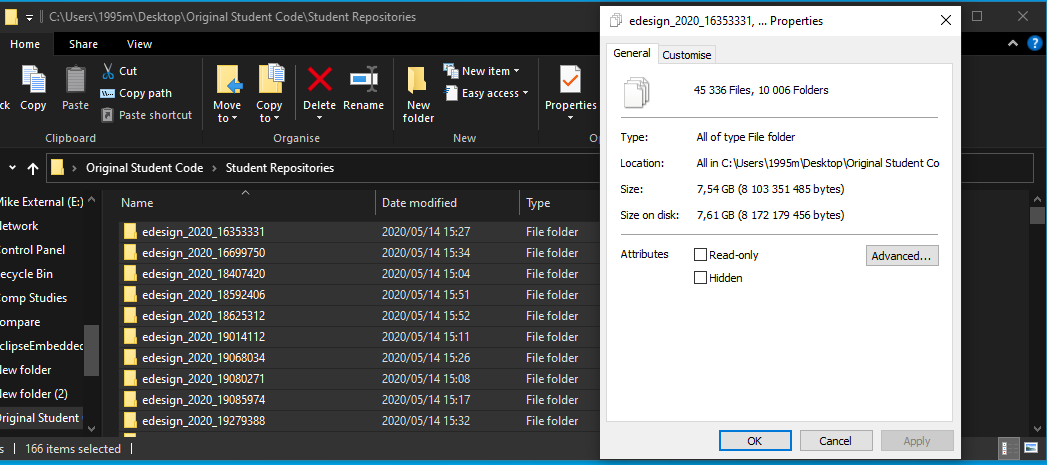
\includegraphics[width = 155mm]{misc1.png}
\caption{Student repository size}
\label{stdSize}
\end{center}
\end{figure}

Figure~\ref{stdSize} illustrates the size and number of files and folders contained within the student repositories of a single year group. It becomes readily apparent that manual code evaluation would be too laborious. An autonomous system is therefore required in order to evaluate student \hyperref[listAbr]{MCU} code.


\section{Autonomous System Outline}
\label{aso}
It has been established that student repositories are too numerous to manually navigate and evaluate. A novel solution is thus required, whereby student code can be evaluated in an autonomous way. 

\begin{figure}[H]
\begin{center}
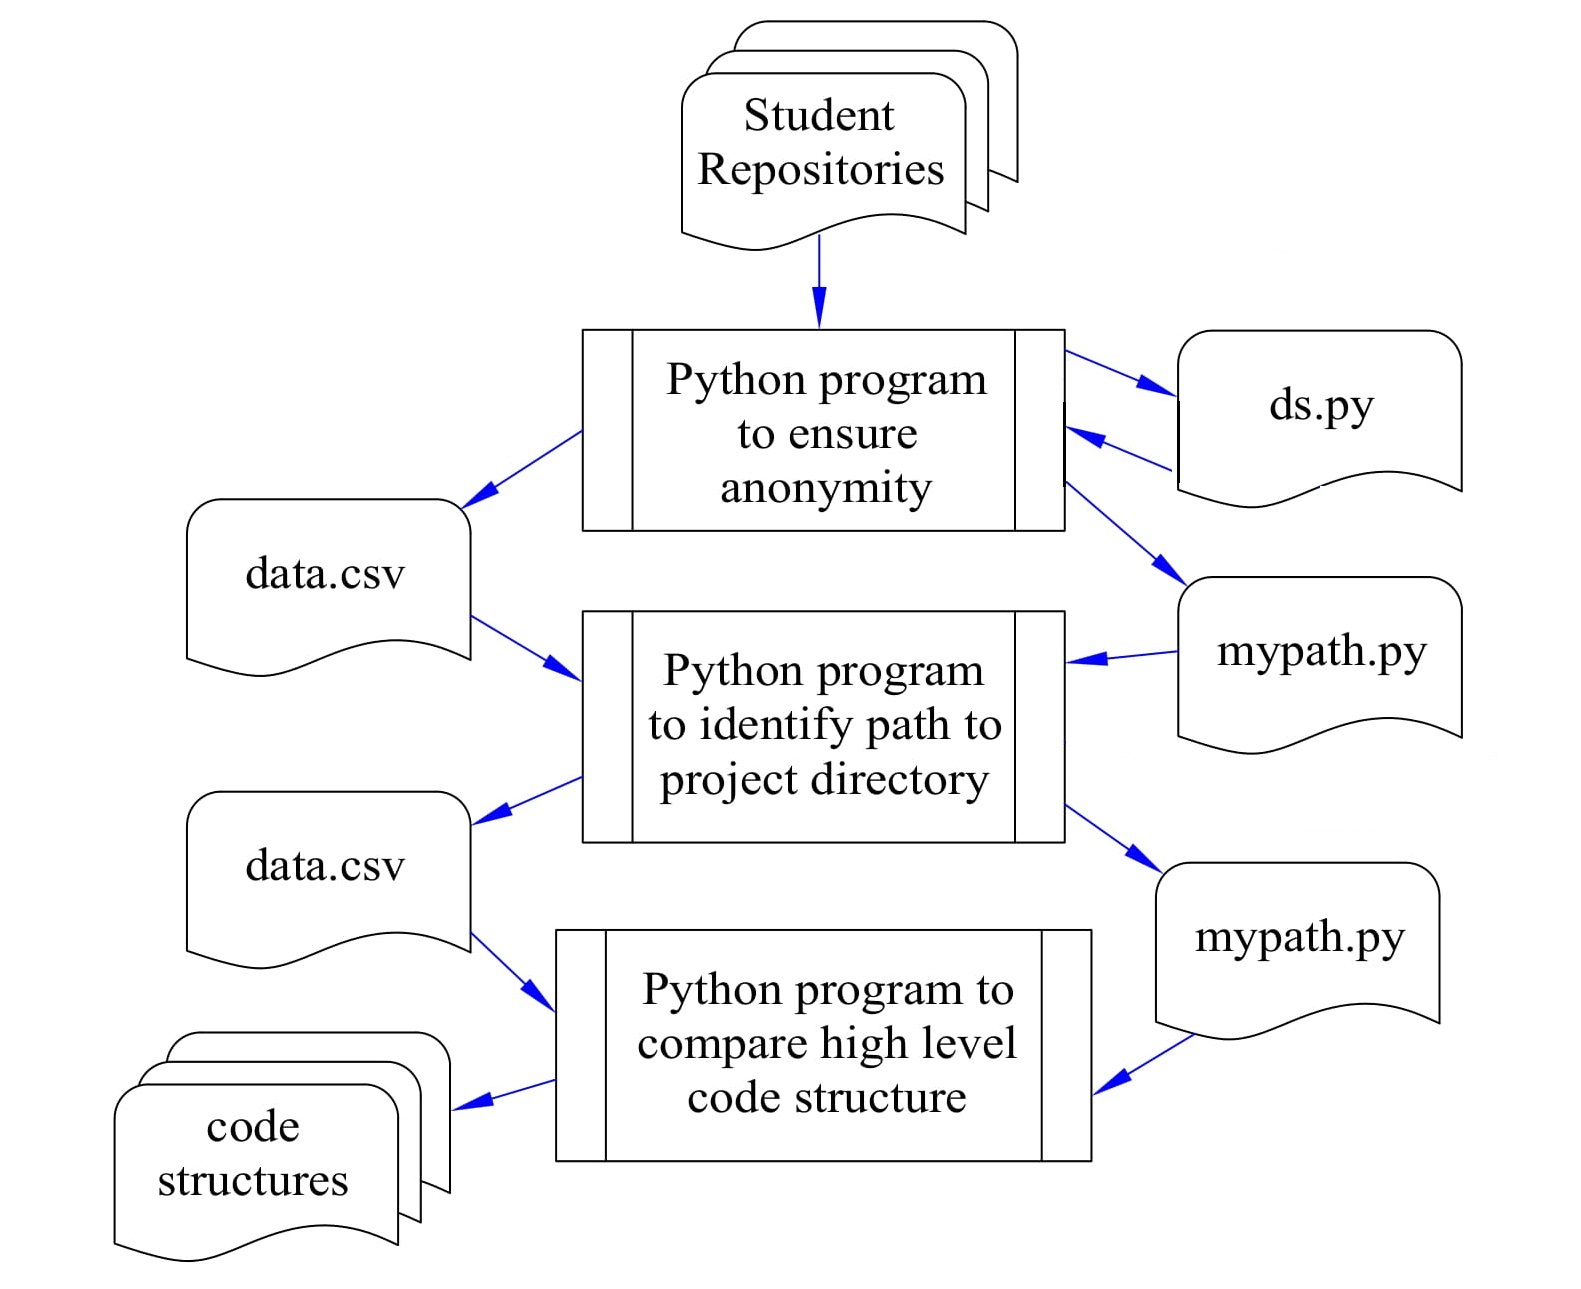
\includegraphics[width = 100mm]{flow2.jpg}
\caption{Autonomous system outline}
\label{aso}
\end{center}
\end{figure}

Figure~\ref{aso} shows the outline of the autonomous system. It can be seen that the program consists of three functional blocks and various inputs and outputs. The reasoning behind these functional block choices will briefly be discussed in the following sections. 


\subsection{Python program to ensure anonymity}
\label{p1}

STM32CubeIDE has a very particular project structure consisting of various directories containing source code, included libraries, drivers and debugger files. These directories are contained within a project root directory and the general structure is highlighted below:

\begin{figure}[H]
\begin{center}
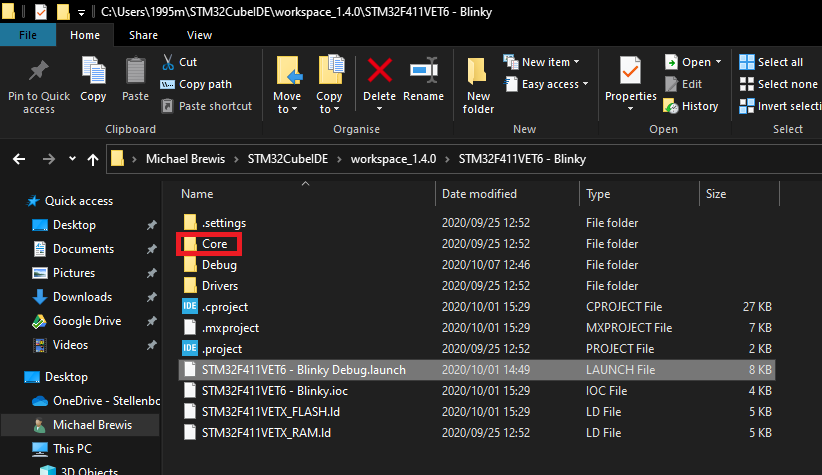
\includegraphics[width = 120mm]{stmProject.png}
\caption{STM32CubeIDE project structure}
\label{stmProj}
\end{center}
\end{figure}

Figure~\ref{stmProj} illustrates the default STM32CubeIDE project outline. It can be seen that any valid project contains a Core folder. This folder contains all the relevant C code and included libraries. It is this folder that is of relevance. The project illustrated above was created in STM32CubeIDE to blink an LED on an STM32F411 \hyperref[listAbr]{MCU}. It is, however, not part of the repositories sent by Dr A Barnard. These repositories are, in fact, not depicted in order to maintain student anonymity. 
\\\\
Anonymity is indeed a very important part of the automation process, when it comes to evaluating student code. Once access to the repositories have been gained, it becomes necessary to remove student numbers from folder and file names. The ethical reason for this is twofold. Firstly, students submit their respective repositories without opting into its use as part of this project. Secondly, this project does not aim to identify cases of plagiarism. If a case of plagiarism is identified as a side effect of the autonomous system, it is vital that these cases cannot be traced back to students.
\\\\
It can be seen that there is only one input to the relevant python script. This input is all the relevant student directories. How the autonomous system identifies these repositories and interacts with them will be discussed in \color{green} section that says how the thing is read\color{black}.
\\\\
It can be observed from Figure~\ref{aso}, that the python script which ensures anonymity has three outputs. The first output is another python script called ds\hyperref[listExt]{.py} which stores the unique identifier associated with a specific student number. As a result the ds\hyperref[listExt]{.py} file generated can be imported by second executions of this program in order to populate the needed data frame (further discussion in \color{green} section that says how the thing is read\color{black}. A second file, namely mypath\hyperref[listExt]{.py}, is also generated. This file is used to store the absolute path of certain directories and files within the project root directory and will be discussed in greater detail in \textbf{\nameref{4detailedd}}. Lastly, the third output is the data\hyperref[listExt]{.csv} file. It is generated within the first script and populated using the ds\hyperref[listExt]{.py} module.

\subsection{Python program to identify path to project directories}
\label{p2}
Once the needed outputs, from the first program, as per Figure~\ref{aso} have been generated, a python program is needed to save the absolute path to the relevant folder within each student repository. This will ensure that the python programs work on any PC and are not relative to the folder hierarchies of the host machine. The absolute path to the needed folders will indeed serve as input to the rest of the programs in the autonomous system depicted in Figure~\ref{aso}.
\\\\
Although it is not immediately apparent that this functional block is prominent enough to be conceptualized as a separate program, this is not the case. The identification of the relevant folder (and contained files) is a cardinal step in the autonomous system. This is because students often submit their projects in such a way, that the project folder is nested within various parent directories. If the rest of the autonomous system is to function correctly, the correct directory must be identified and its absolute path stored. Moreover, the aforementioned functionality should be maintained regardless of multiple nested directories.
\\\\
It can be seen form Figure~\ref{aso} that the functional block discussed in this subsection receives, as inputs, the outputs generated by the program discussed in \textbf{\ref{p1} \nameref{p1}}. Firstly, the mypath\hyperref[listExt]{.py} module is needed to navigate the folder directories on the host machine as saved by the first program. Next, the data\hyperref[listExt]{.csv} file is required to link student repositories with unique identifiers as assigned by the first program. This file will, additionally, be modified by the program discussed in this subsection, to store the absolute path to the pertaining project folder.  

\subsection{Python program to evaluate high-level code structures}
\label{p3}

The final program in the execution chain of the autonomous process creates files for comparison. It receives the outputs of the previous python programs. The function of this step in the autonomous process, is to identify and extract student created configurations, both in STM32CubeIDE created files as well as the students main\hyperref[listAbr]{.c} file.
\\\\
To begin with, this program will receive the data\hyperref[listExt]{.csv} file (modified by previous steps in the automation process). The data\hyperref[listExt]{.csv} file, at this point, will contain all the needed paths to student specific project repositories on the host machine. It is, moreover, required to assure that repositories are valid and that student numbers have been linked to unique identifiers. This program will, furthermore after execution, delete the data\hyperref[listExt]{.csv} file to ensure that students are not implicated in cases of plagiarism. The ethical reasons for this are discussed in \textbf{\ref{p1} \nameref{p1}}. The aforementioned functionality can easily be omitted if cases of plagiarism are indeed to be detected. 
\\\\
In addition to the data\hyperref[listExt]{.csv} file, this program also receives, as input, the mypath\hyperref[listExt]{.py} module. This is, once again, needed in order to produce the outputs of the program in the correct directory on the host PC.

\subsection{Autonomous process directory structure}
\label{p4}
In the previous subsections, the autonomous process has been outlined. The outputs produced by each of the steps in this process has also been discussed. This subsection will highlight the folder structure produced and utilized by the relevant system. Due to the modular nature of the autonomous system, the outputs of one process are often the inputs to another. Furthermore, the programs have been written in such a way that multiple executions of a single process are often necessitated \color{green} as dicussed in detailed part \color{black}.
\\\\
It therefore becomes necessary to store these outputs and inputs in a common directory, to be accessed by any iteration of the various steps in the process. The figure below illustrates these directories.

\begin{figure}[H]
\begin{center}
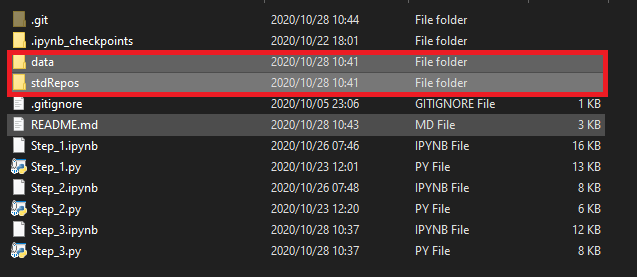
\includegraphics[width = 155mm]{dir.png}
\caption{Pertaining autonomous process directories}
\label{dir}
\end{center}
\end{figure}

Figure~\ref{dir} illustrates the two directories produced by the autonomous process. This will be discussed in greater detail in \color{green} detailed part\color{black}. It can be seen from the figure that "stdRepos" and "data" are produced as two directories. Within the "stdRepos" directory, the various student repositories are to be placed by the user of the host machine. The subsequent steps in the autonomous process will access the "stdRepos" directory and the various nested folders within. These nested folders are depicted in the following figure:

\begin{figure}[H]
\begin{center}
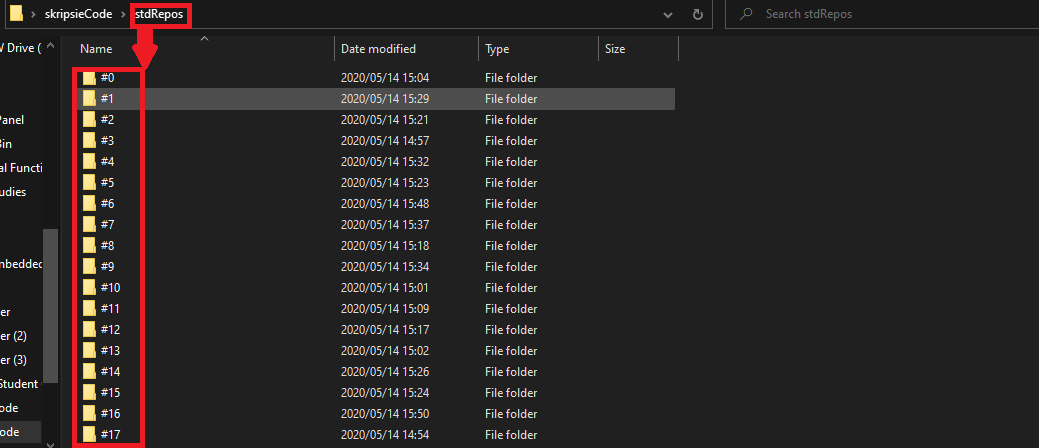
\includegraphics[width = 155mm]{stdRepos.png}
\caption{Content of the stdRepos folder}
\label{stdRepos}
\end{center}
\end{figure}

Figure~\ref{stdRepos} depicts the content of the stdRepos folder, after the program discussed in \textbf{\ref{p1} \nameref{p1}}, has executed.
\\\\
In addition to the previously discussed repository a "data" repository is also created by the process in discussion. This repository will serve as a common storage location for any programs that form part of the system. Within this directory the output files of the final step are stored, as well as the required python modules created by the system. The contents of the "data" folder are partially displayed in the following figure:

\begin{figure}[H]
\begin{center}
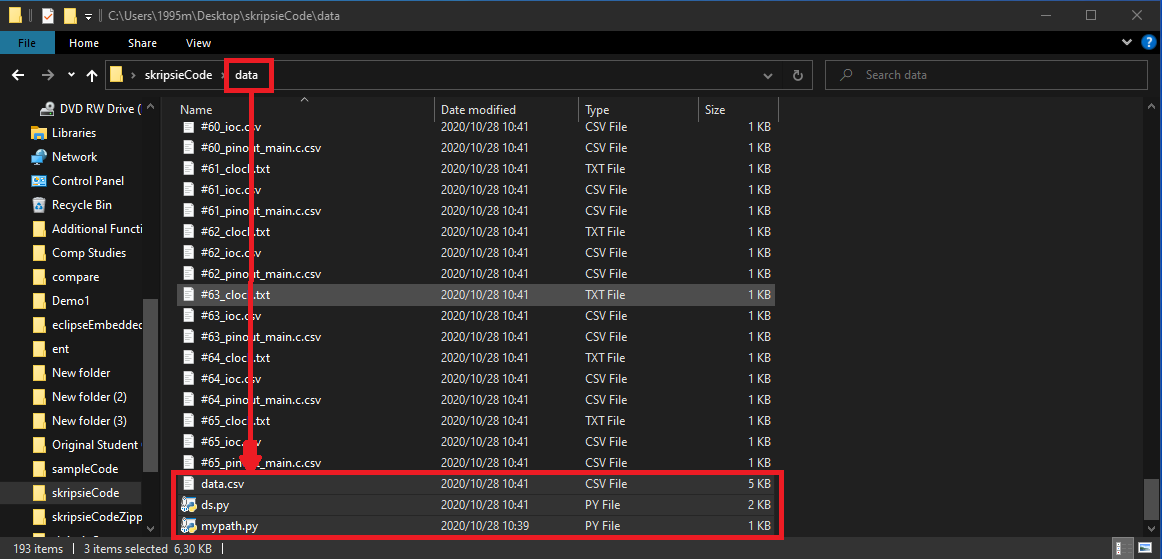
\includegraphics[width = 155mm]{data.png} 
\caption{Content of the data folder}
\label{data}
\end{center}
\end{figure}

Figure~\ref{data} depicts the content of the data folder, after all the programs discussed in \textbf{\ref{aso} \nameref{aso}}, has executed. It can be seen that the pertaining python modules (namely mypath\hyperref[listExt]{.py} and ds\hyperref[listExt]{.py}) as well as the data\hyperref[listExt]{.csv} is contained within this repository. In addition to these files, the various student structures are also stored in this folder (discussed in \color{green} that part \color{black}). The various functional blocks depicted in Figure~\ref{stdRepos}, will have access to the respective directories using the mypath\hyperref[listExt]{.py} module in the "data" directory.
\\\\
This subsection concludes the outline of the autonomous system and provides a general overview of the system. In the following chapter each of the functional blocks discussed in \textbf{\ref{p1} \nameref{p1}}, \textbf{\ref{p2} \nameref{p2}} and \textbf{\ref{p3} \nameref{p3}} will be expanded upon.
